\documentclass[a4paper,openright,12pt]{report}
\usepackage[spanish]{babel}
\usepackage[utf8]{inputenc}
\usepackage{cite}
\usepackage{graphicx}
\usepackage{pdfpages}
\usepackage{fancyhdr}
\usepackage{hyperref}
\hypersetup{
	colorlinks,
	citecolor=black,
	filecolor=black,
	linkcolor=black,
	urlcolor=black
}

\begin{document}
\renewcommand{\listtablename}{Índice de tablas}


%título

\begin{titlepage}

\AddToShipoutPicture*{\put(0,0){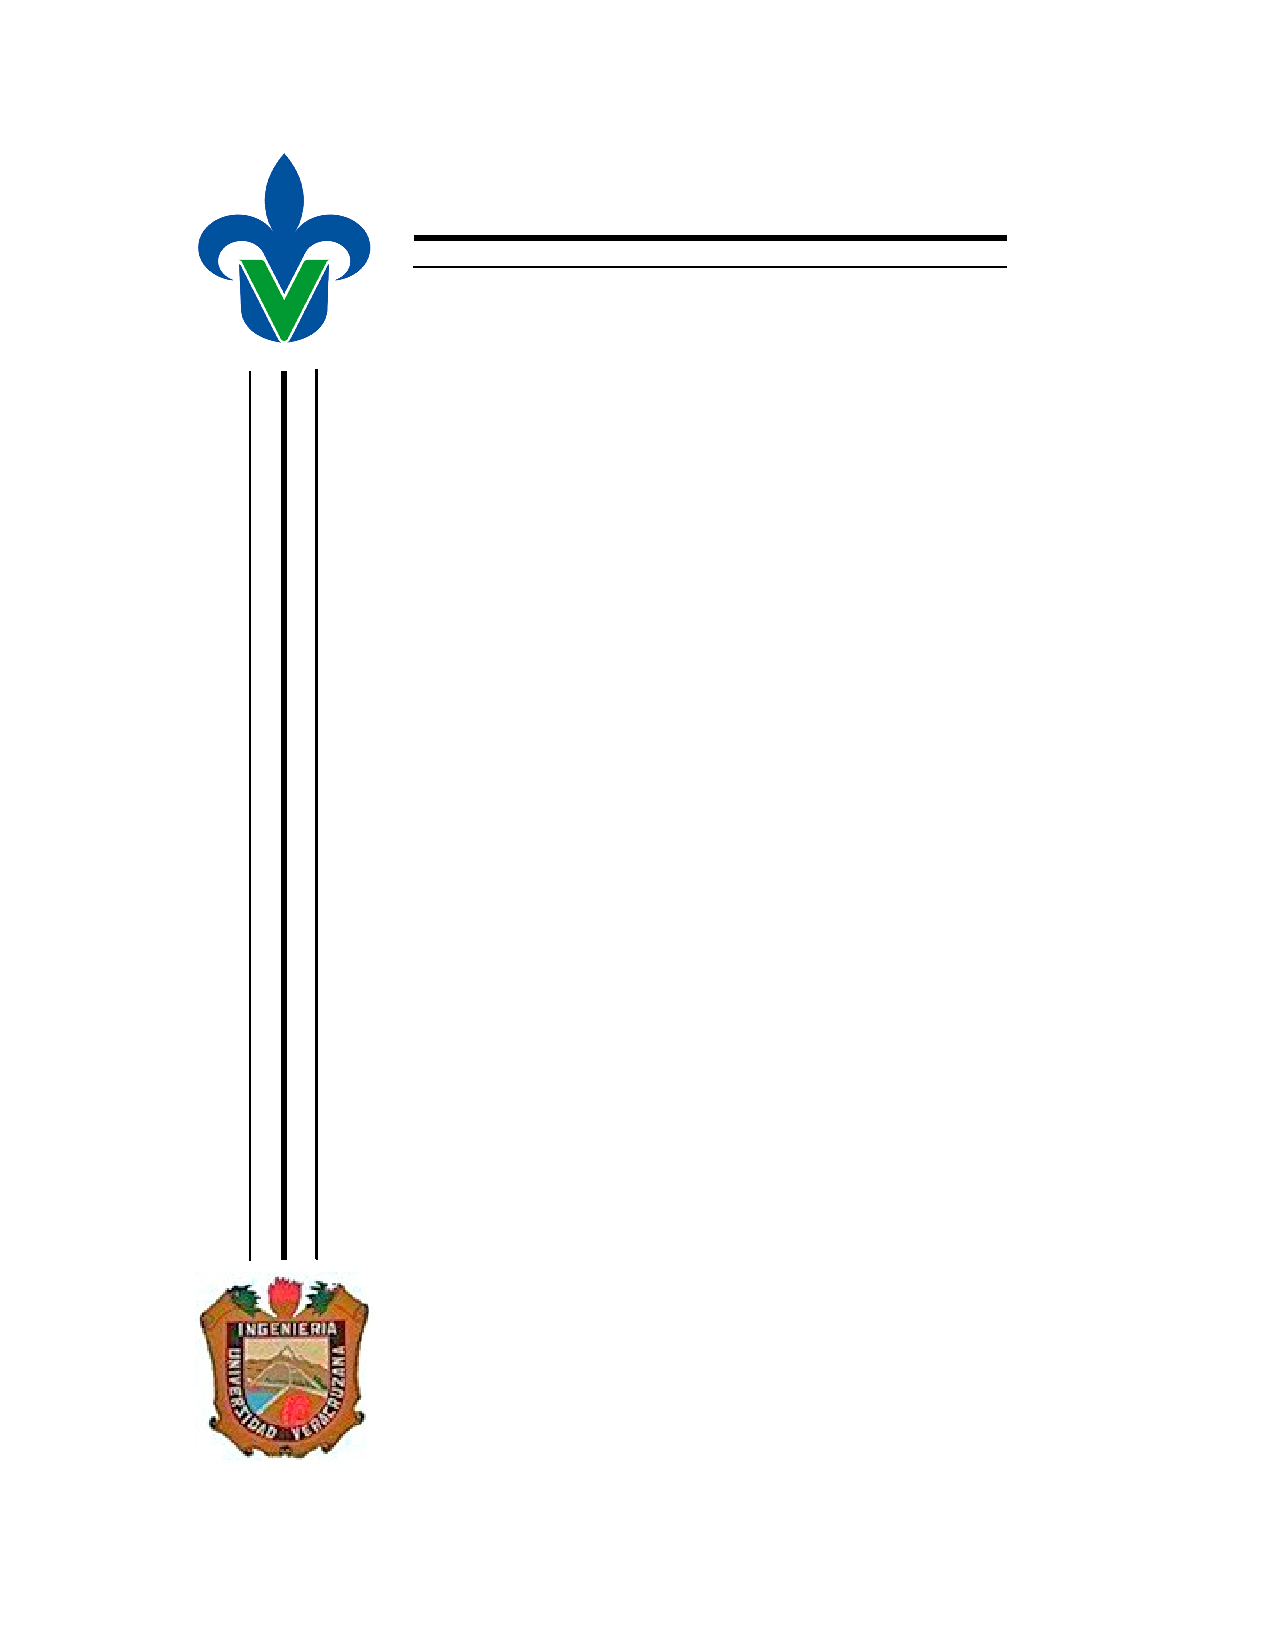
\includegraphics[scale=1]{portada2.pdf}}} % Image background
	
	\begin{minipage}[t][1.75cm][b]{1.15\textwidth}
		\begin{center}
			\begin{Large}
				\textsc{Universidad Veracruzana}
			\end{Large}	
			\\
			\vspace*{0.6cm}
			\textsc{Facultad de Ingeniería}
		\end{center}
	\end{minipage}
\hspace*{3.6cm}
\mbox{	
\begin{minipage}[b][6cm][b]{0.7\textwidth}
	\begin{center}
		\begin{LARGE}
			\textsc{Proyección Adaptativa de un
				escenario 3D basado en la
				perspectiva de una persona}
		\end{LARGE}	
		
	\end{center}
\end{minipage}
	}
	\\
\hspace*{3.6cm}	
	\mbox{	
		\begin{minipage}[b][7.5cm][b]{0.7\textwidth}
			\begin{center}
					\textsc{
						\large Que para obtener el grado de:\\
						\small
						Ingeniero en Informática\\
						\large Presenta:\\
						\small Yadira Fleitas Toranzo\\
						\vspace*{1cm}
						\large Asesor de tesis:\\
						\small	Dr. Luis Felipe Marín Urías
						}
			\end{center}
		\end{minipage}
	}
	\\
	\hspace*{3.6cm}	
	\mbox{	
		\begin{minipage}[b][3cm][b]{0.7\textwidth}
			\begin{center}
				\textsc{
				\begin{small}
					Boca del Río, Veracruz, Junio de 2017
				\end{small}	
				}
			\end{center}
		\end{minipage}
	}
	

\end{titlepage}
%%%%%%

%%%DEDICATORIA%%%
\chapter*{}
\pagenumbering{Roman}
\begin{flushright}
\textit{Dedicado a...\\ blablabla}
\end{flushright}
%%%%%%%%%%%%%%%%

%%%AGRADECIMIENTOS Y RESUMEN%%%
\chapter*{Agradecimientos}
\addcontentsline{toc}{chapter}{Agradecimientos}

¡Muchas gracias a todos jijiji!

\chapter*{Resumen}
\addcontentsline{toc}{section}{Resumen}

Una bonita historia jejeje
%%%%%%%%%%%%%%%%%%%%%%%%%%%

%%%ÍNDICE DE CONTENIDOS%%%
\tableofcontents
\cleardoublepage
\addcontentsline{toc}{chapter}{Lista de figuras}
\listoffigures
\cleardoublepage
\addcontentsline{toc}{chapter}{Lista de tablas}
\listoftables

%%%%%%%%

\cleardoublepage
%%%CAPÍTULO 1 -> INTRODUCCIÓN
\chapter{Introducción}\label{cap.introduccion}
\pagenumbering{arabic}
\pagestyle{fancy}
Vivimos en una época en la cual la tecnología forma parte esencial de nuestras vidas. En donde el ser humano, es capaz de mejorar y optimizar su entorno con el objetivo de satisfacer cada una de sus necesidades. El alcance que ha tenido la tecnología digital, nos abre camino para el surgimiento de nuevas técnicas capaces de colaborar en el desarrollo de múltiples áreas o disciplinas, ayudando a la creación de distintas formas para facilitar su aprendizaje, optimización y avance de las mismas.\\
Así, la tecnología digital ha servido de apoyo incluso en situaciones en donde el ser humano requiere de entrenamiento para realizar ciertas actividades peligrosas, costosas o difíciles de ejecutar y que son proporcionadas a través de entornos virtuales, para mejorar sus habilidades y evitar a todo costo el riesgo de perder incluso vidas humanas. Una aplicación que ejemplifica claramente lo mencionado, lo tenemos en los simuladores de vuelo, que lo que se intenta hacer es replicar la experiencia de pilotar una aeronave de la manera más realista posible. No obstante, el desarrollo e implementación de simuladores de este tipo, implica la fabricación de cabinas en tamaño real con accionadores hidráulicos o electromecánicos, el cual conlleva un gran costo de los mismos.\\
Es por ello que con el objetivo de minimizar costos y de no requerir de tantos equipos para la inmersión a estos escenarios artificiales, existe una rama de la tecnología conocida como Realidad Virtual (VR, Virtual Reality), que sustituye nuestro mundo real a través de dispositivos que nos permitan encontrarnos en otro lugar, es decir, sumergirnos en una realidad que no existe. Tomando el ejemplo anterior, se han estado desarrollando simuladores a través de este tipo de tecnología, con el objetivo de ahorrar recursos y que se puedan disponer de una manera más rápida y frecuente \cite{Pausch1992}.\\
Los dispositivos utilizados para visualizar este tipo de Realidad Virtual, son conocidos como HMD (del inglés head-mounted display), similares a un casco, que reproducen imágenes sobre una pantalla muy cercana a nuestros ojos, permitiendo abarcar todo el campo de visión del usuario y así brinden una inmersión de éste en un mundo ficticio.\\
Igualmente, existen algunos HMD’s que son utilizados por otro tipo de tecnología basada en entornos virtuales y que adopta el nombre de Realidad Aumentada.\\
AR (del inglés Augmented Reality), es una tecnología que intenta lograr perfeccionar nuestra propia realidad, combinando nuestro mundo real con el virtual que, a diferencia de la Realidad Virtual, que crea todo un entorno artificial desde cero, éste tipo de tecnología agrega elementos virtuales a una realidad que ya existe.\\
Hoy en día, la Realidad Aumentada ha adquirido mayor popularidad y expansión debido a las aplicaciones en donde se encuentra. Por ejemplo, en la industria del entretenimiento, específicamente en el área de los videojuegos, existe una aplicación muy popular, conocida como Pokémon GO \cite{Dorward2017}, el cual consiste en la búsqueda y captura de personajes de la saga Pokémon, que se encuentran escondidos en el mundo real, visualizados a través de un smartphone, en donde claramente se puede ver el concepto de Realidad Aumentada debido a que los personajes están superpuestos en nuestro mundo real. Así mismo, encontramos que la AR abarca áreas como la medicina \cite{Marescaux2004,Ploder1995}, turismo \cite{Kounavis2012}, manufactura \cite{Frund2004}, entre muchas otras.\\
Todas estas aplicaciones en donde se encuentra la Realidad Aumentada, son visualizadas a través de dispositivos tales como HMD (Hololens de Microsoft, GoogleGlass de Google), computadoras, tablets o smartphones, y aunque gradualmente se han ido optimizando tanto el hardware como el software de cada uno de ellos, su uso impide al observador tener una conexión más real con su mundo, debido a factores tales como el campo de visión limitado por los mismos dispositivos, latencia en los gráficos que en ocasiones puede provocar mareos, y la necesidad obligatoria de llevar un equipo encima para poder visualizar este tipo de realidad. Debido a lo anterior, existe una variante de ésta tecnología, conocida como Realidad Aumentada Espacial (SAR, Spatial Augmented Reality), que mantiene el mismo concepto de la AR, pero con la diferencia que ésta es mostrada mediante proyectores digitales, es decir, proyecta información u objetos virtuales directamente sobre objetos físicos, por lo tanto, ya no necesitaríamos llevar con nosotros algún dispositivo para visualizarla.\\
En un inicio, SAR, simplemente se utilizaba en la proyección de imágenes o videos que se adaptaban a la forma de fachadas de edificios ofreciendo espectáculos visuales. Pero más adelante se integró la fase de interacción con estos elementos virtuales, lo cual aunque ayudó a involucrarse en varias industrias y expandir su aplicación, aumentó su nivel de complejidad, encontrando varias problemáticas que actualmente siguen en proceso de desarrollo.
%%->Planteamiento del problema
\section{Planteamiento del problema}
La Realidad Aumentada Espacial (SAR), siendo entonces un nuevo paradigma que se deriva de la Realidad Aumentada, es una nueva forma de visualizar elementos virtuales sin la necesidad de verlos a través de dispositivos sujetos a estar en nuestro cuerpo.\\
Estos objetos virtuales proyectados en nuestro entorno, a pesar de jugar en algunos casos con nuestra mente, para dar un efecto 3D, utilizando sombras en lugares específicos y aplicando técnicas para dar profundidad, se puede lograr distinguir de lo real con sólo situarnos en otro lugar en torno a la proyección y verlo desde otra perspectiva. Esto ocasiona por lo tanto que exista aún una gran barrera entre lo que es real y lo que es virtual en términos de SAR.\\
El estudio de proyectar objetos virtuales 3D, que se asemejen tanto a los objetos físicos, pudiendo en algunas ocasiones sustituirlos, es una de las problemáticas actuales sin resolver y que muy pocos han intentado abordar, debido al grado de complejidad que pudiese tener el desarrollo de ésta. Considerando que, para que se pueda implementar esta mejora, se debe tener en cuenta varios aspectos tales como:
\begin{itemize}
\item La deformación de los objetos virtuales al proyectarse directamente sobre los objetos físicos.
\item La detección de una o más personas.
\item El seguimiento de la persona a la cual se le tomará en cuenta la perspectiva, debido a que únicamente se podría proyectar la perspectiva de una sola persona.
\item La calidad de la proyección de los elementos virtuales.
\end{itemize}
Se propone, por lo tanto, a través de un esquema simple inicial y en un futuro, aplicable a cualquier escenario virtual, la proyección de un escenario con elementos 3D, adaptable a la perspectiva de la persona, perfeccionando y cumpliendo aún más con el objetivo del término de Realidad Aumentada Espacial.
%%

%%Justificación
\section{Justificación}
Aunque varios proyectos en donde se aplica SAR, se encuentran dirigidos a la industria de los videojuegos (lo cual, a pesar de lo que muchos opinan ser una pérdida de tiempo, éstos son capaces de desarrollar múltiples habilidades en los usuarios y vivir experiencias únicas), el uso de SAR, se expande a distintas áreas proporcionando enriquecer la experiencia visual, y por lo tanto apoyando el desarrollo y entendimiento de las mismas.\\
Es por ello que proyectar escenarios u objetos virtuales cambiando su ángulo de vista cuando una persona se mueve alrededor de éste, nos brinda la oportunidad de darle más realidad a un objeto virtual y vivir una experiencia mejorada de SAR.\\
En la educación el uso de esta técnica nos permitiría, agilizar el proceso de aprendizaje, debido al impacto que causaría la proyección de objetos virtuales 3D, en temas como figuras o lugares históricos, planetas, el cuerpo humano, entre otros, que dieran la posibilidad de mostrar más información de la proporcionada en una simple imagen, y así motivar su estudio.\\
En la rama de la arquitectura, la visualización de una estructura, ya sea un edificio o casa, proyectada en 3D sin la necesidad de crear una maqueta, ayudaría a ahorrar recursos y vivir la misma experiencia, incluyendo la ventaja de poder modificar su modelado y ver instantáneamente el resultado que obtendrían de manera virtual.\\
Por lo tanto, el desarrollo de mostrar un escenario virtual 3D, según la perspectiva de una persona, sería un paso más hacia la adaptabilidad de un mundo virtual en el mundo real, siendo una potente herramienta de visualización capaz de contribuir en el desarrollo de múltiples áreas.
%%

%%Objetivos
\section{Objetivos}
%General
\subsection{General}
Desarrollar un sistema capaz de determinar el ángulo correspondiente de un entorno virtual basado en la perspectiva de una persona y proyectarlo en nuestro mundo para proporcionar un efecto de realidad.
%
%Específicos
\subsection{Específicos}
\begin{itemize}
\item Determinación de los módulos que intervendrán en el sistema mediante el análisis de los requerimientos.
\item Detección del número de personas en la escena y selección del individuo de interacción, por medio del desarrollo y la implementación de un módulo.
\item Determinar la posición en donde se encuentre la persona y la altura proporcionada por la imagen de profundidad de un sensor RGB - D, por medio del desarrollo e implementación de un módulo.
\item Optimización del sistema por medio de una comparativa de diversas técnicas en cada uno de los módulos del sistema.
\end{itemize}
%
%%

%%Hipótesis
\section{Hipótesis}
Basado en la posición y altura de una persona, obtenidas mediante un sensor RGB – D es posible obtener su perspectiva respecto a un entorno virtual que será proyectado y creará el efecto 3D que tanto se intenta conseguir.
%%
%%%%%%%%%%%%%%%%%%%%%%%%%%%%%%%%%%%%%%%%%%%%%%%%%%%%%%%%%%%%

%%%CAPÍTULO 2 -> MARCO TEÓRICO%%%
\chapter{Marco Teórico}\label{cap.marcoteorico}
Dado que el presente trabajo de tesis, se centrará en el área de la Realidad Aumentada Espacial (SAR), específicamente en la optimización de la proyección de objetos virtuales 3D, será necesario establecer algunas terminologías y trabajos relacionados que sirvan de apoyo para el correcto entendimiento de éste.
%%Antecedentes
\section{Antecedentes}
La Realidad Aumentada (AR) técnicamente hablando se puede definir como la tecnología capaz de superponer objetos o información virtual en una secuencia de imágenes capturadas en tiempo real de nuestro propio entorno, creando la ilusión de que ambos mundos (virtual y real) se fusionan en uno, es decir, creando una realidad mixta (MR).\\
La capacidad de proporcionar una experiencia visual tal para el usuario, que pueda llegar a pensar que éstos forman parte de su realidad, es uno de los retos que intenta conseguir la Realidad Aumentada (AR).\\
La forma tradicional de visualizar este tipo de tecnología, es a través de dispositivos tales como HMD’s, lentes, computadoras, tablets o smartphones, (en inglés See-through Augmented Reality, STAR \cite{Sol2016}), y aunque cada vez surgen mas aplicaciones entorno a estos artefactos, el uso de ellos impide al observador tener una conexión mas real con su mundo, debido principalmente al campo de visión limitado por los mismos.\\
La Realidad Aumentada Espacial (SAR), es una variante de la AR, que muestra mediante proyectores digitales, información u objectos virtuales directamente sobre objetos físicos, lo cual una de las ventajas que trae consigo con respecto a STAR, es el hecho de no tener que llevar un equipo encima para poder visualizar este tipo de realidad e involucrar la capacidad de poder interactuar directamente (sentido del tacto) de tal modo que nos ayude a estar mas en contacto con los objetos virtuales.\\
En sus inicios, su desarrollo se basaba en resolver básicamente problemas en cuanto a la distorsión de la imagen en la irregularidad de la superficie, pero luego se implementó la fase de interacción entre el usuario y los elementos virtuales, surgiendo problemas mas complejos que aún siguen en proceso de desarrollo.\\
Dependiendo del uso o la aplicación en donde se encuentre ésta tecnología, se le atribuyen otros nombres que ayuden a entender mas su propósito en donde se esté implementando, ésto debido a que cuando hablamos de ``Espacial'', no solo nos estamos refiriendo a la percepción de información adicional a través del sentido visual, sino que también podemos involucrar el tacto y el sentido auditivo.\\ 

\subsection{Projection mapping}
Comercialmente SAR, también es conocida como ``projection o video mapping'', refiriéndose a la proyección de información virtual en objetos reales, con el objetivo de enriquecerlos visualmente, proyectando una nueva forma de percibir el objeto. De igual manera se pueden proyectar imágenes o elementos virtuales en superficies tales como paredes de edificios para publicidad, como medio artístico en escenarios o incluso en el rostro o cuerpo de las personas.\\
Su nivel de complejidad, por lo tanto, varía dependiendo de la superficie en donde pueda ser proyectada la información. Por ejemplo, inicialmente, en proyectos como Luminous Room \cite{Under1997} se proyectaba la información en una superficie plana, donde únicamente se ajustaba la deformación que ocasionaba la proyección dependiendo de donde se encontrara el proyector. Sin embargo, años antes, ya se tomaba en cuenta en cuenta la estructura del escenario \cite{Dorsey1991} (en éste caso pantallas curvas) para proyectar información, en donde generaban las imágenes pre-distorsionadas para que luego se pudiese visualizar de la forma correcta. En cambio, cuando la superficie en donde se proyecta la información posee objetos y por lo tanto se muestra de forma irregular, se requiere un análisis previo de su forma para así capturar la información 3D de los objetos físicos, pre-distorsionar la imagen conforme a la irregularidad del escenario, tomar en cuenta la posición en donde se encuentra la persona y seguido a esto, la proyección correcta de los elementos virtuales \cite{Raskar1998b,Raskar2001,Starner2003,Wilson2007}.
\subsection{Interacción en SAR}
En sus primeros años de desarrollo, analizado en la sección anterior, no se contaba con una fase de interacción entre el usuario y los elementos virtuales, debido a que su propósito en ese momento, era mostrar información adicional, aumentando la experiencia visual. Fue entonces, que gracias a grandes compañías como Microsoft Research, desarrollaron proyectos y propusieron nuevas técnicas que incluían la interacción a través de las manos, el seguimiento de la cabeza o el cuerpo, lo cual propició la expansión de SAR en distintas áreas, principalmente en el aprendizaje y entretenimiento.\\
Mucho de este desarrollo y avance se inició a través de proyectos que mostraban la información en sobremesa (tabletop). Éstas eran visualizadas a través de proyectores que generalmente estaban ubicados arriba de la mesa (front-projected displays) o debajo de ésta (técnica conocida como retroproyección).\\
Con referencia a la proyección frontal, ésta daba como resultado que las manos u otra parte del cuerpo de las personas, obstruían la proyección, ocasionando poca realidad de inmersión de elementos virtuales en nuestro entorno\cite{dietz2001}. Como solución a éste problema, MirageTable\cite{bibid} proyecto desarrollado por Microsoft Research, propone un modelo de detección de manos para mostrar información virtual sin la distorsión que causaría esta.

 a  o bien, se econtraba abajo para que el usuario no obstruyera la proyección en caso de incluir las manos, utilizando la retroproyección (rar-projected displays).

%%
%%Esto del Arte
\section{Estado del arte}
El estudio de la toma de perspectiva, es muy reciente.
todavía nada aquí ):
%%
%%%%%%%%%%%%%%%%%%%%%%%%%%%%%%%%%%%%%%%%%%%%%%%%%%%%

%%%CAPÍTULO 3 -> DISEÑO%%%
\chapter{Dise\~no}\label{cap.diseno}
aún nada...
%%%%%%%%%%%%%%%%%%%%%%%%%%%%%%%%%%%%%%%%%%%%%%%%%%%%%%%

%%%CAPÍTULO 4 -> IMPLEMENTACIÓN Y RESULTADOS%%%
\chapter{Implementación y resultados}\label{cap.implementacionyresultados}
tampoco nadita ):
%%%%%%%%%%%%%%%%%%%%%%%%%%%%%%%%%%%%%%%%%%%%%%%%%%%%%%%%

%%%CAPÍTULO 5 -> CONCLUSIONES%%%
\chapter{Conclusiones}\label{cap.conclusiones}
y con esto concluímos /O/ 
\section{Trabajo Futuro}
muchos xD
%%%%%%%%%%%%%%%%%%%%%%%%%%%%%%%%%%%%%%%


%%%BIBLIOGRAFÍA%%%
\cleardoublepage
\addcontentsline{toc}{chapter}{Bibliografía}
\bibliographystyle{acm}
\bibliography{biblio}



\end{document}